\subsection{Switch Matrix :}
Automotive BMS applications demand sophisticated and robust switch matrices, as in the market there are no switch matrix will available according to the application. There has been specific knowledge used to pick this switching component. Switching components are more unlikely than the conventional components, such a vote for picking the switching components always registered for the high power MOSFETs because of various technological advantages over conventional electro-mechanical switches. Since the component choice is entirely left to the design engineer, it is always a good practice to design these switch matrix boards from scratch to have full control over the system. The following sections will give more insights into the switch matrix.
\begin{figure}[h]
	\centering
	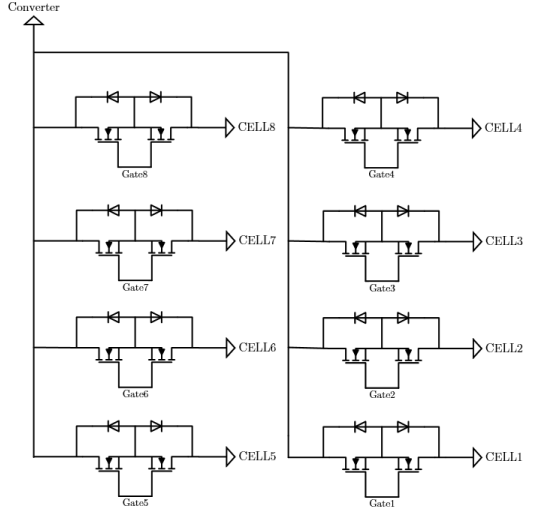
\includegraphics[width=0.8\textwidth]{Chap04/Figures/switch_matrix.PNG}
	\caption{Typical Mosfet switch matrix for 8 batteries \cite{Active_Balancing_Thesis_Raber} }
	\label{fig:Mosfet_Switch_Matrix}
\end{figure}
\indent Single or double back-to-back FETS are used for the switch matrix, back to back MOSFETS are two MOSFETs housed in a single package or externally by connecting the gates of FETs are common. The Figure\ref{fig:Mosfet_Switch_Matrix} implicates one such example of a switch matrix using the back-to-back MOSFETs.

\subsubsection{The initiative understanding behind choosing the switch matrix MOSFET:}
\begin{itemize}
    \item Low Rds ON; low on-state resistance implicates that MOSFET can carry high DC with lower dissipation.
    \item High Blocking voltage; High blocking voltage between the drain and the source ensures the breakdown safety of the MOSFET against the full Battery pack voltage.
    \item Low gate area - to drive the FET faster, and it cost less than the current budget for the FET's gate driver.
    \item Low gate drive voltage. So-and-so forth.
\end{itemize}

\noindent By analyzing the criteria mentioned in the section, the choice is made to use STD20NF06L for the switch matrix. The component specification is as follows :
STD20NF06\cite{Switch_MatrixFET_STD20NF06L} is the high-power MOSFET that has been developed for automotive applications to handle the High current with very low input gate capacitance. The FET has perfect dv/dt. STD20NF06 is DPACK package which is quite big compared to SMD package and single package dual back-to-back FET's, yet the FET is opted for because of the following benefits. The back-to-back FET arrangement is made externally as shown in Figure \ref{fig:Mosfet_Switch_Matrix}.
for more insights into the component refer to the MOSFET Datasheet \cite{Switch_MatrixFET_STD20NF06L}.
	


\begin{center}
\begin{tabular}{ |p{4cm}|p{4cm}|p{4cm}|p{4cm}|  }
\hline
\multicolumn{4}{|c|}{STD20NF06L Datasheet} \\
\hline
Symbol& Parameter &Value & Unit \\
\hline
$V_{ds}$  & Drain-source voltage & 60 & V \\
$V_{gs}$  & Gate-source voltage  & $\frac{+}{-}$ 18 & V \\
$I_{d}$   & Drain current (continuous) at $ TC = 25 \deg C$ & 24 & A \\
$P_{Tot}$ & Total power dissipation at $ TC = 25 \deg C$    & 60 & W \\
$\frac{dv}{dt}$ & Peak diode recovery voltage slope    & 10 & $V/ns$ \\
$C_{iss}$ & Input capacitance VDS = 25 V, f = 1 MHz, VGS = 0 V, & 660 & C \\
$R_{ds(on)}$ & Static drain-source on-resistanc & @VGS = 10V,@ID = 12A, 32  & $\Omega$ \\
\hline
\end{tabular}
\end{center}